\documentclass[10pt]{article}

\usepackage{fancyhdr}
\usepackage{graphicx}
\usepackage{geometry}
\usepackage{lastpage}
\usepackage{titling}
\usepackage{sectsty}
\usepackage{setspace}
\usepackage{changepage}
\usepackage[shortlabels]{enumitem}
\usepackage{subcaption}
\usepackage{helvet}
\usepackage{hyperref}

\usepackage{tabularx}
\usepackage[table]{xcolor}
\usepackage{array}
\newcolumntype{P}[1]{>{\centering\arraybackslash}p{#1}}

\usepackage{siunitx}
\usepackage{nicefrac}
\usepackage{amsmath}
\usepackage{gensymb}
\usepackage{amssymb}
\usepackage{float}
\setcounter{MaxMatrixCols}{11}
\usepackage{indentfirst}

\usepackage{listings}
\usepackage{matlab-prettifier}
% \usepackage{color}
% \definecolor{dkgreen}{rgb}{0,0.6,0}
% \definecolor{gray}{rgb}{0.5,0.5,0.5}
% \definecolor{mauve}{rgb}{0.58,0,0.82}

\lstset
{
  frame=tb,
  style=Matlab-editor,
  % language=MATLAB, %Matlab-editor,
  aboveskip=3mm,
  belowskip=3mm,
  showstringspaces=false,
  columns=flexible,
  basicstyle={\small\ttfamily},
  numbers=none,
  % numberstyle=\tiny\color{gray},
  % keywordstyle=\color{blue},
  % commentstyle=\color{dkgreen},
  % stringstyle=\color{mauve},
  breaklines=true,
  breakatwhitespace=true,
  tabsize=3
}

\geometry
{
  letterpaper, 
  total={175.9mm,229.4mm}, 
  top=25mm, 
  left=20mm, 
  headheight=15pt,
  voffset=12pt,
  footskip=15pt
}
\author{Daniel Sturdivant}
\title{Homework 3}
\date{April 2023}
\graphicspath{ {./media/} }

\pagestyle{fancy}
\fancyhead[R]{April 10, 2023}
\fancyhead[L]{Sturdivant, Daniel}
\fancyhead[C]{MECH 7710 Optimal}
\fancyfoot[C]{Page \thepage\ of \pageref{LastPage}}

\makeatletter
\def\@maketitle
{
  \null
  \begin{center}
    {\huge \@title \\}
  \end{center}
  \vskip 5mm
}
\makeatother

\sectionfont{\fontsize{16}{16}}
\subsectionfont{\fontsize{13}{13}\normalfont}
\renewcommand{\thesubsection}{\arabic{section}-\arabic{subsection}}
\renewcommand{\familydefault}{\sfdefault}
\newcommand{\solution}{\textbf{Solution: \\}}


%% ========================================================================== %%
\begin{document}

\maketitle
\thispagestyle{fancy}
\setstretch{1.25}
% \setlength{\parskip}{0em}
% \setlength{\abovedisplayskip}{-8pt}
% \setlength{\belowdisplayskip}{12pt}
\setlength{\parindent}{0pt}

\begin{enumerate}[label=\textbf{\arabic*.}]
  \itemsep 24pt
  % PROBLEM 1
  \item Kalman Filter at its best – simulation (actually the Kalman filter is 
  also quite reliable when we have an excellent model and low noise sensors). 
  Suppose we have a $2^{nd}$ order system that we are regulating about zero 
  (position and velocity) by wrapping an "optimal" control loop around the 
  system. The new dynamics of the continuous time system are given by the 
  closed-loop $A$ matrix:
  \begin{equation*}
    A_{cl} = 
    \begin{bmatrix}
      0 & 1 \\ -1 & -1.4
    \end{bmatrix}
  \end{equation*}
  Suppose our measurement is simply position ($C=\begin{bmatrix} 1 & 0 
  \end{bmatrix}$). There is a white noise process disturbance (force, $B_w = 
  \begin{bmatrix} 0 & 1 \end{bmatrix}^T$) acting on the controlled system.
  \begin{enumerate}[(a)]
    \itemsep -2pt 
    \item Simulate the controlled system with the disturbance force 
    ($1\sigma=2$) and a sampled sensor noise ($1\sigma=1$) for 100 seconds at a 
    10 Hz sample rate.

    \item What is $Q$, $Q_d$ and $R_d$?
    
    \item Calculate the steady state Kalman gain for the system. This can be 
    done in one of many ways: iterate the kalman filter until it converges, 
    dlqe.m, dare.m, kalman.m, dlqr.m (+ predictor to current estimator trick), 
    etc. What is the steady state covariance of the estimates after the time 
    update, $P^{(-)}$, as well as after the measurement update, $P^{(+)}$. 
    Where are the poles of the estimator?

    \item Now use the steady state kalman filter to generate an estimate 
    ($\hat{x}$ and $\hat{\dot{x}}$) of the 2 states over time. Calculate the 
    norm of the standard deviation of the errors for each state.
    \begin{equation}
      N = \sqrt{( std(\dot{x} - \hat{\dot{x}}) )^2 + ( std(x - \hat{x}) )^2}
      \label{eq:1.7}
    \end{equation}

    \item Change the ratio of the $Q_d$ and $R_d$ weights in the Kalman filter 
    design (repeat \emph{part d} with the new Kalman gain but \textbf{DO NOT} 
    regenerate a new $x$ and $\dot{x}$) and determine the effect on the 
    estimation errors. For what ratio of $Q_d$ to $R_d$ are the errors 
    minimized? Note: Often in practice we do not know the actual $Q_d$ and 
    $R_d$, so these tend to be "tuning" parameters we can use to tune our 
    filter. However, according to Kalman the estimation errors are only 
    minimized if we use the $Q_d$ and $R_d$ of the physical system.
  \end{enumerate}
  \vspace{10pt}

  \solution
  % 1.A
  To simulate the system we can use the continuous model in \emph{Equation 
  \ref{eq:1.1}} and evaluate over 100 seconds.
  \begin{equation}
    \begin{split}
      \dot{x} &= A_{cl} x + B_w w \\
      y &= C x + \nu
    \end{split}
    \label{eq:1.1}
  \end{equation}
  Where $x$ contains the states of position and velocity, $\dot{x}$ is the 
  rate of change in these systems, $w$ is the disturbance force or process 
  noise, and $\nu$ is the measurement noise. \emph{Figure \ref{f:1.1}} shows 
  the simulated system.
  \begin{figure}[H]
    \centering
    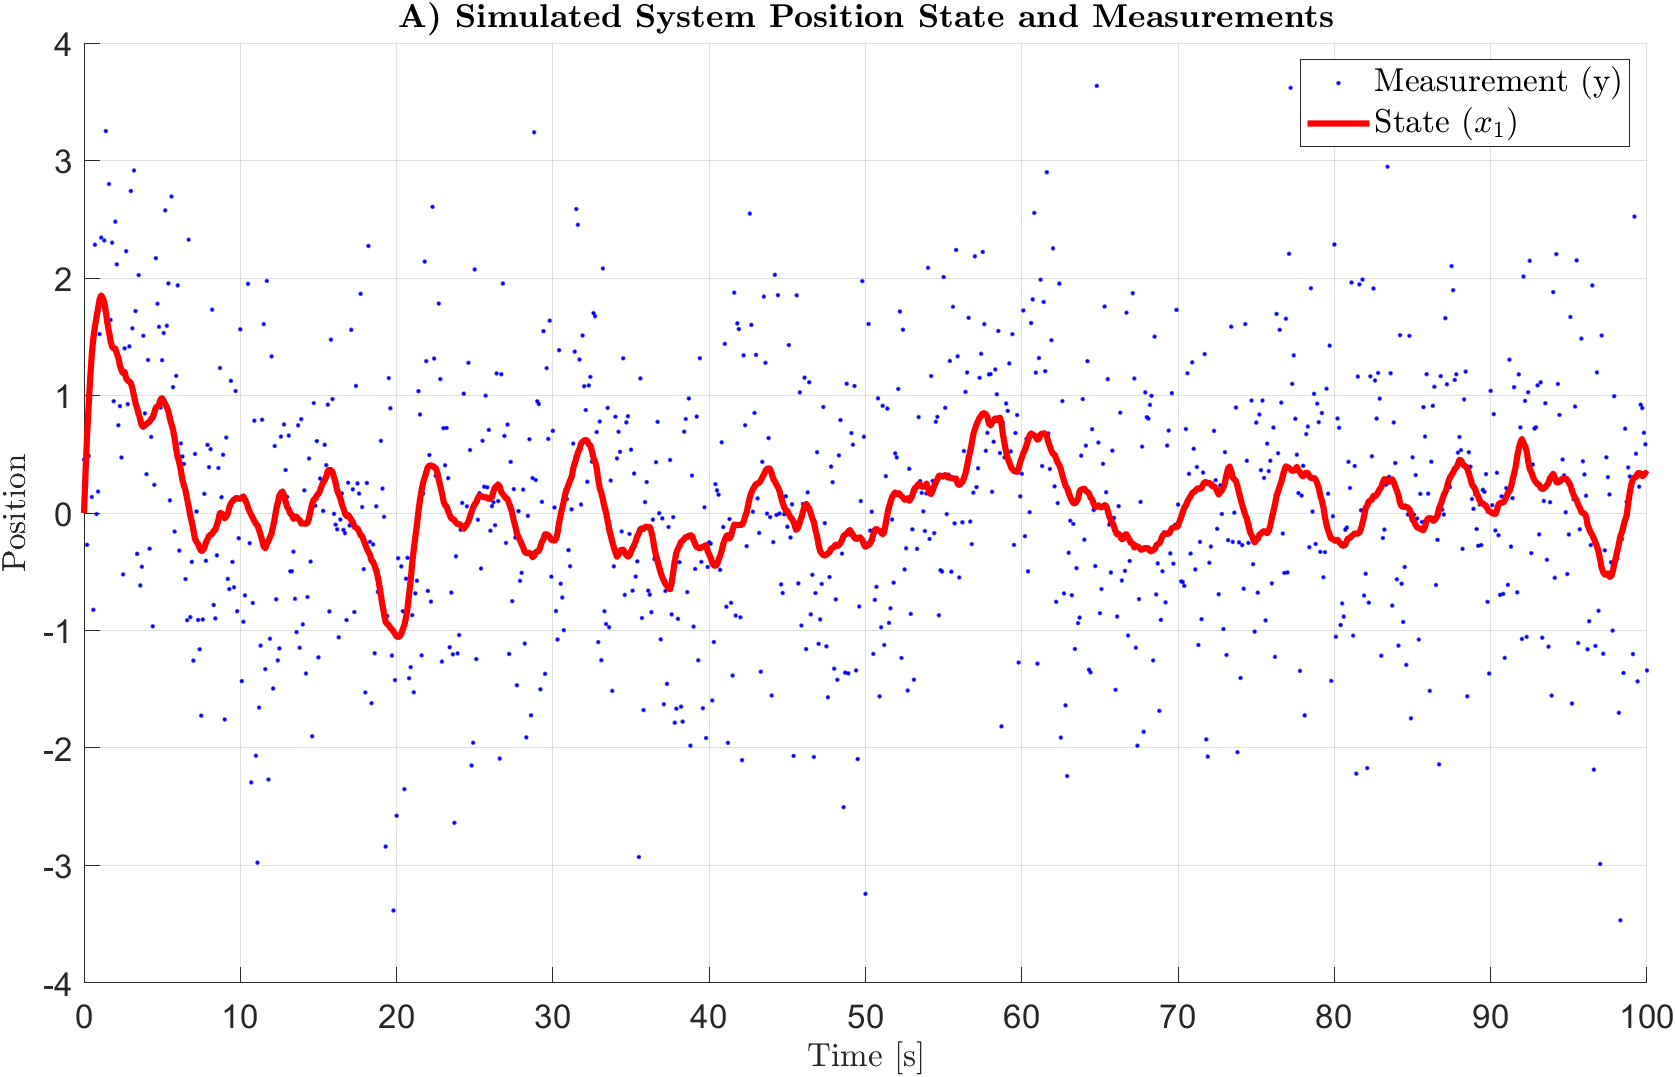
\includegraphics[width=0.8\textwidth]{p1_a.png}
    \caption{Simulated System Position with Measurements.}
    \label{f:1.1}
  \end{figure}

  % 1.B
  Using the desired continuous noise characteristics (\emph{Equation 
  \ref{eq:1.2}}):
  \begin{equation}
    \begin{split}
      Q_c &= 2^2 = 4 \\
      R &= 1^2 = 1   
    \end{split}
    \label{eq:1.2}
  \end{equation}
  Discretizing the system can be done using \emph{Equation \ref{eq:1.3}}, 
  known as Bryson's Trick.
  \begin{equation}
    \begin{split}
       s &= \begin{bmatrix} -A & B_w Q_c B_w^T \\ 0 & A^T \end{bmatrix} \\
       c &= e^{s \Delta t} \\
       A_d &= c[2,2]^T \\
       Q_d &= A_d c[1,2]
    \end{split}
    \label{eq:1.3}
  \end{equation}
  Applying this trick to the system:
  \begin{equation*}
    \begin{split}
      s &= \begin{bmatrix} 0 & -1 & 0 & 0 \\ 1 & 1.4 & 0 & 4 \\ 
                           0 & 0 & 0 & -1 \\ 0 & 0 & 1 & -1.4 \end{bmatrix} \\
      c &\approx eye(4) + s \Delta t =
      \begin{bmatrix} 1 & -0.1 & 0 & 0 \\ 0.1 & 1.14 & 0 & 0.4 \\ 
                      0 & 0 & 1 & -0.1 \\ 0 & 0 & 0.1 & 0.86 \end{bmatrix} \\
      A_d &= \begin{bmatrix} 1 & 0.1 \\ -0.1 & 0.86 \end{bmatrix} \\
      Q_d &= \begin{bmatrix} 0 & 0 \\ 0 & 0.344 \end{bmatrix}
    \end{split}
    \label{eq:1.4}
  \end{equation*}
  Since $R$ is measurement noise, it does not change via discretation and can 
  be assumed equivalent to the continuous measurement noise.\\

  % 1.C
  In order to determine the steady-state Kalman Gain and Covariance, the time 
  and  measurement updates must be implemented 
  (\emph{Equation \ref{eq:1.5}}).
  \begin{equation}
    \begin{split}
      &\text{\bf{Time Update}} \\
      &x_k^- = A_d x_{k-1}^+ \\
      &P_k^- = A_d P_{k-1}^+ A_d^T + Q_d \\
      &\text{\bf{Measurement Update}} \\
      &L_k = P_k^- C^T (C P_k^- C^T + R)^{-1} \\
      &P_k^+ = (I - L_k C) P_k^- \\
      &x_k^+ = x_k^- + L_k (y_k - C x_k^-)
    \end{split}
    \label{eq:1.5}
  \end{equation}
  Running the Kalman Filter until it reaches steady state results in 
  \emph{Figure \ref{f:1.2}}, which includes values of $L_{ss}$, $P_{ss}^-$, 
  and $P_{ss}^+$.
  \begin{figure}[H]
    \centering
    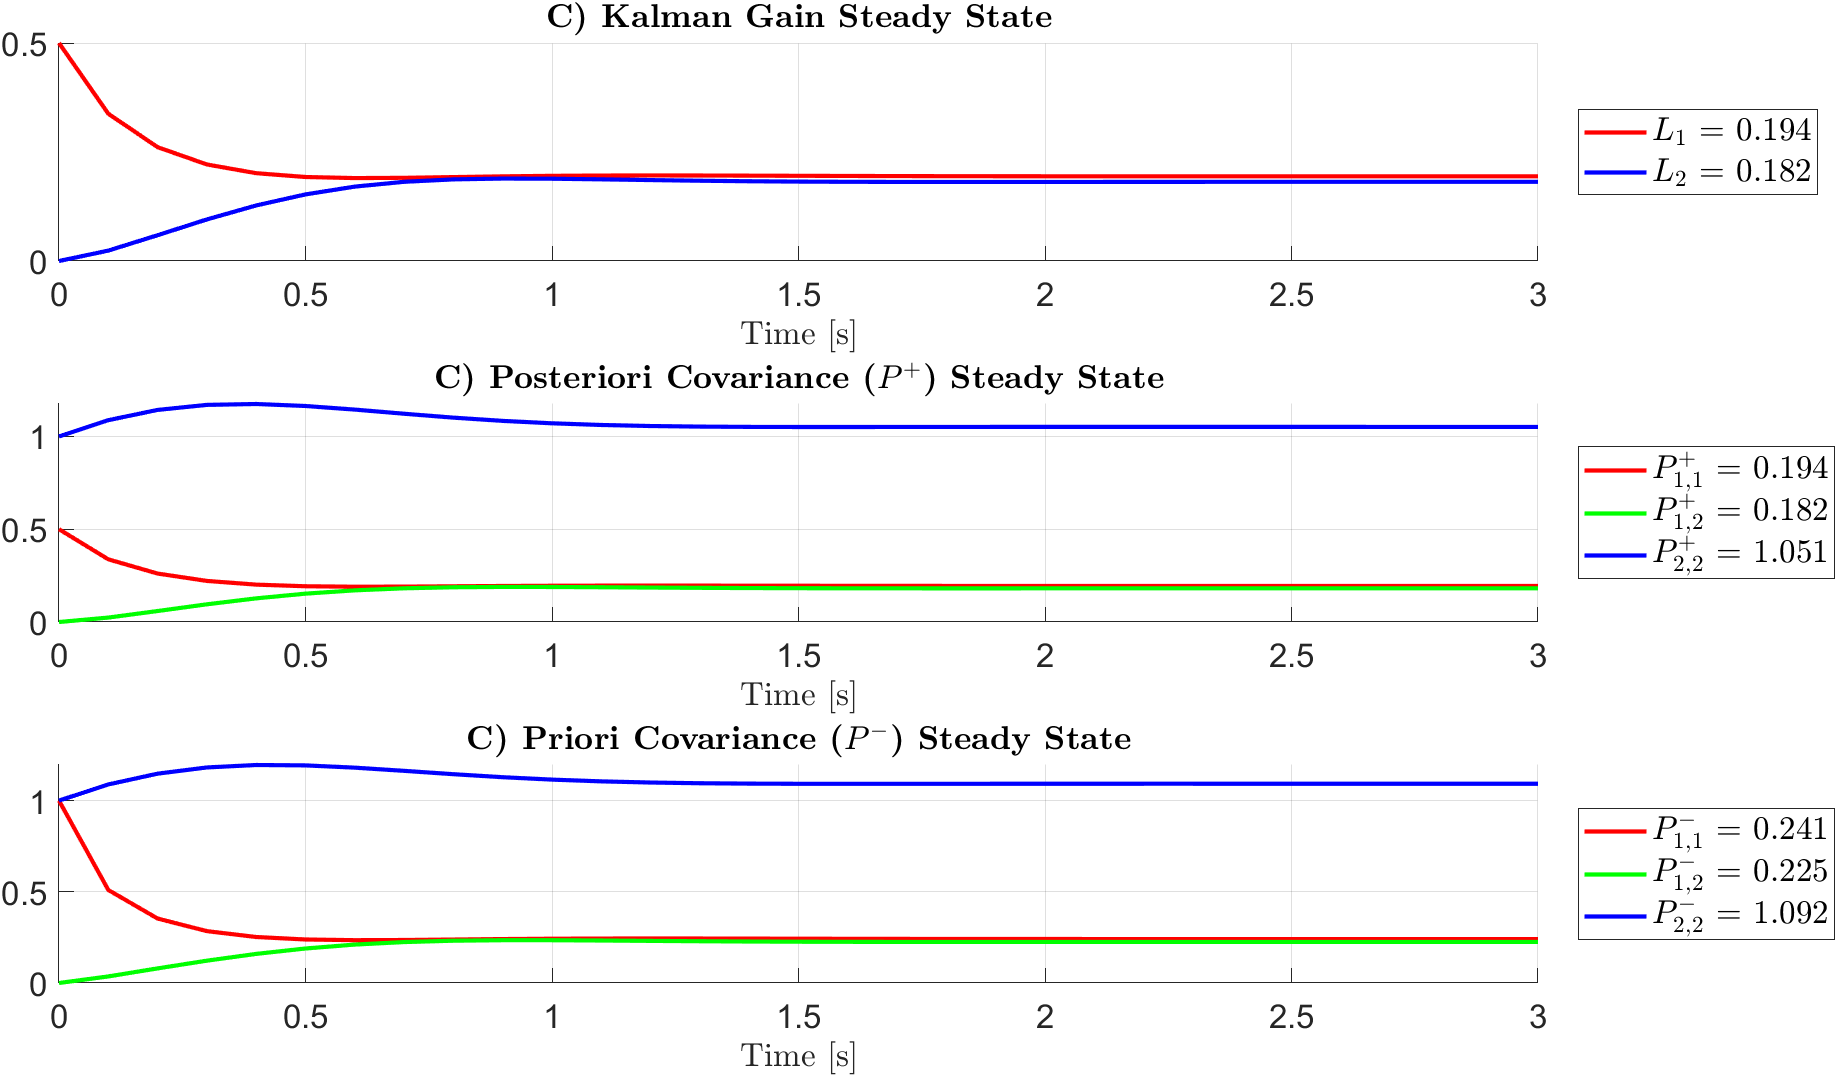
\includegraphics[width=0.8\textwidth]{p1_c.png}
    \caption{Kalman Filter Values vs. Time.}
    \label{f:1.2}
  \end{figure}
  To find the poles of the new system, the determinant of the new closed-loop 
  system must be evaluated as follows:
  \begin{equation}
    \begin{split}
      0 &= det(s - (A_{cl}-L_{ss}C)) \\
      s &= \begin{bmatrix} 0.833+0.166i \\ 0.833-0.166i \end{bmatrix}
    \end{split}
    \label{eq:1.6}
  \end{equation}

  % 1.D
  The position estimate of the Kalman Filter is shown in \emph{Figure \ref{f:1.3}}.
  \begin{figure}[H]
    \centering
    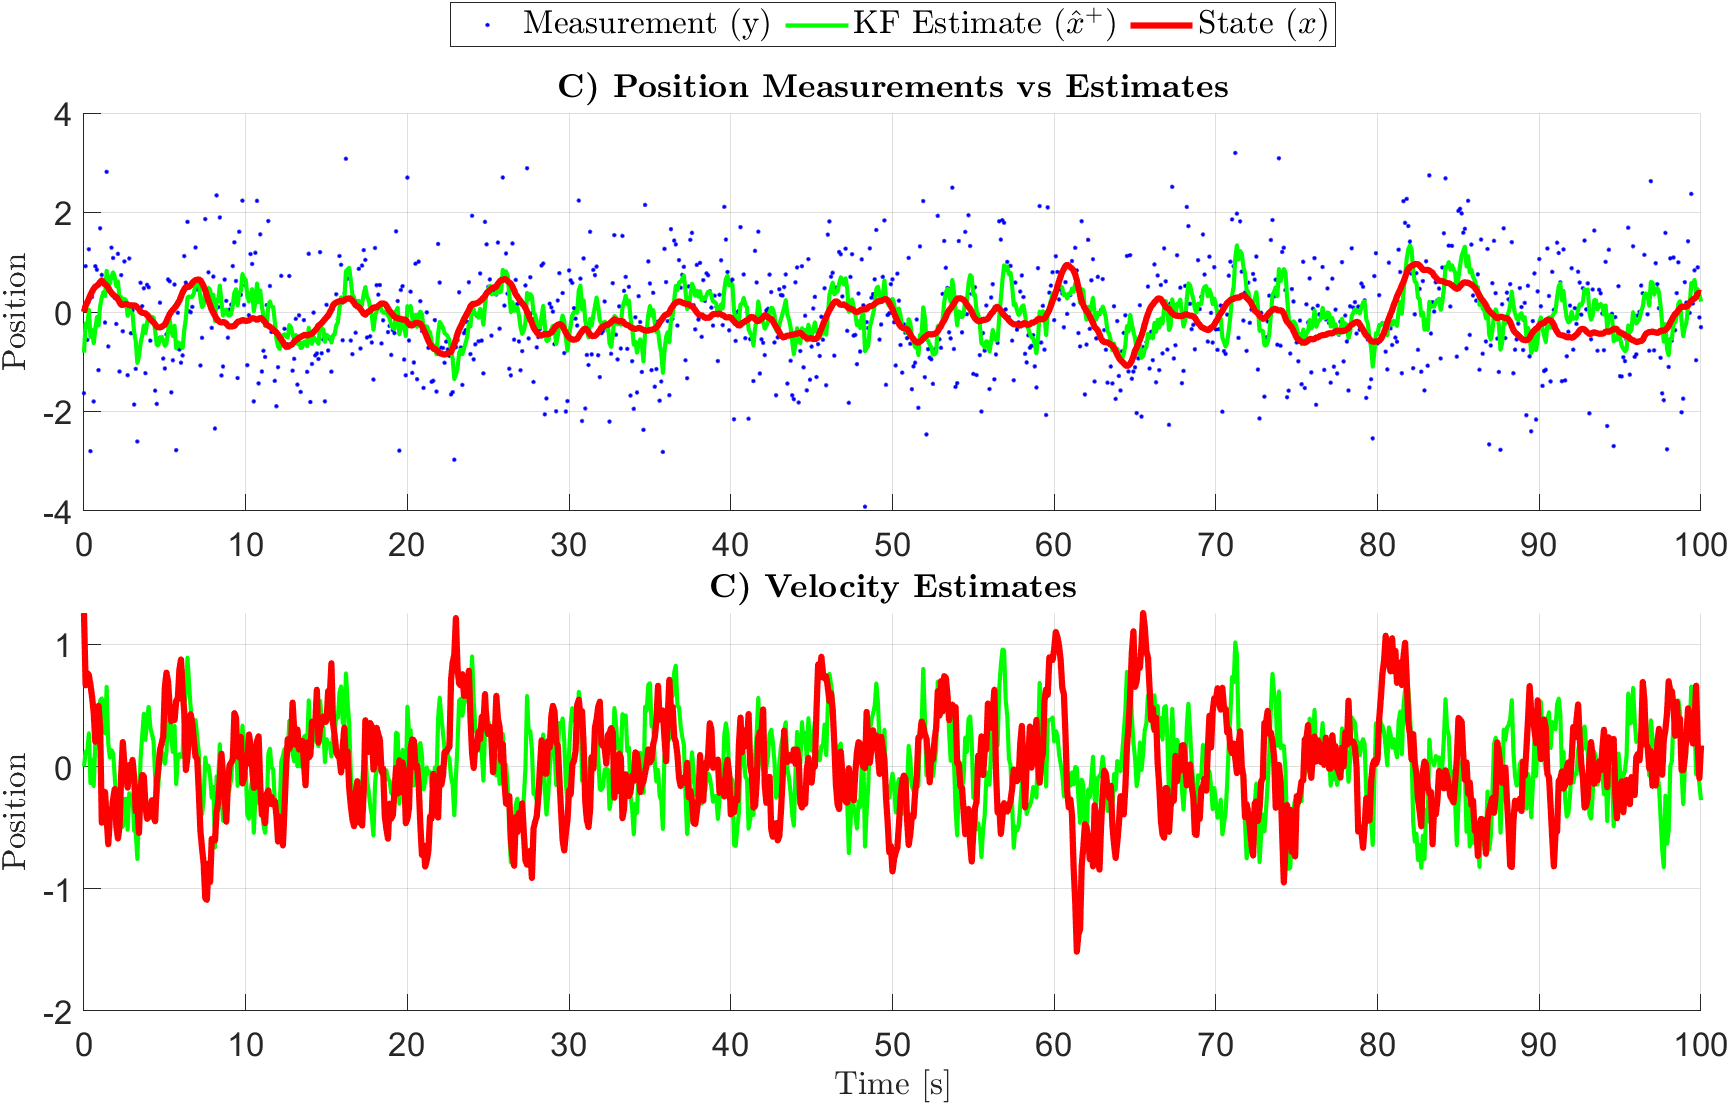
\includegraphics[width=0.8\textwidth]{p1_c2.png}
    \caption{Filtered Position Solution.}
    \label{f:1.3}
  \end{figure}
  Applying \emph{Equation \ref{eq:1.7}} to the difference between the states of 
  the simulated system and the Kalman Filter estimation results in a normalized 
  standard deviation of $N=0.609$. \\

  % 1.E
  To find the optimal ratio of measurement to process noise, measurement noise 
  was kept constant, $R=1$, and the process noise was changed on a log scale from 
  $10^{-6} \leftrightarrow 10^{6}$ such that the ratio between the values changed on each 
  iteration. A graphical representation is shown in \emph{Figure \ref{f:1.4}}.
  \begin{figure}[H]
    \centering
    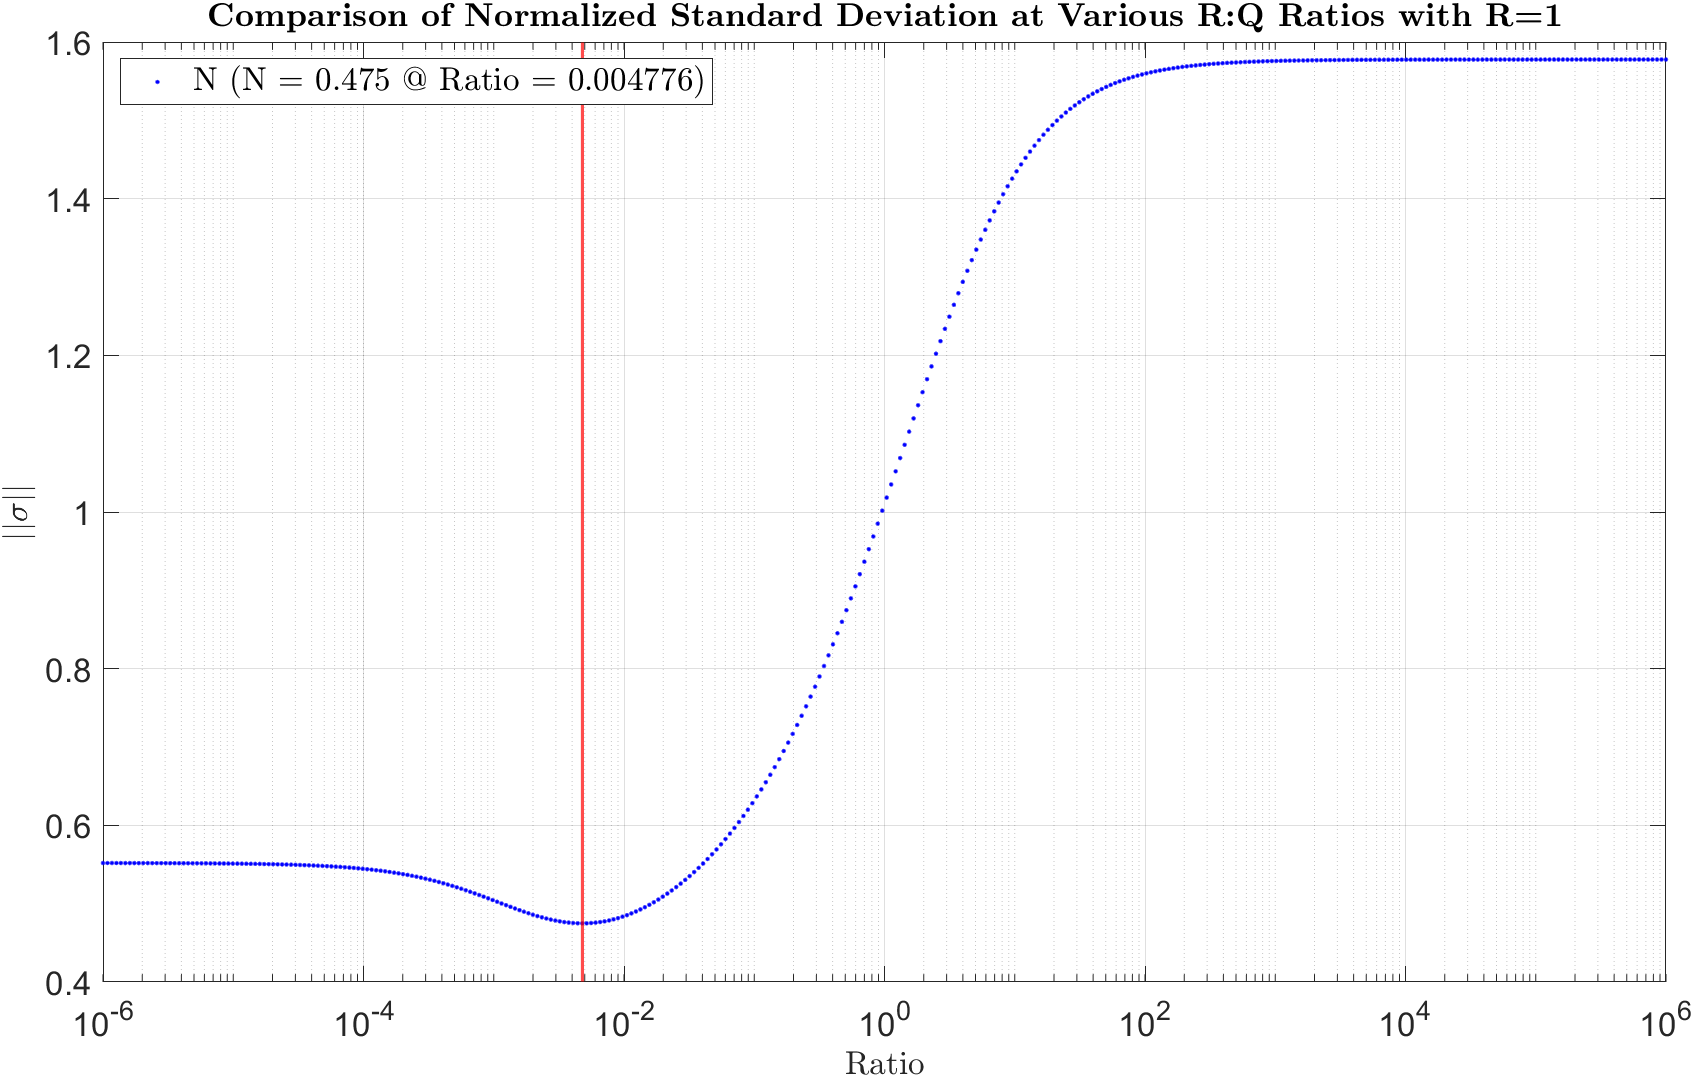
\includegraphics[width=0.8\textwidth]{p1_e.png}
    \caption{Normalized Standard Deviation at Different R to Q Ratios.}
    \label{f:1.4}
  \end{figure}
  As shown in the \emph{Figure \ref{f:1.4}}, the optimal ratio occurs at 
  $R:Q=0.0056$ with a normalized standard deviation of $N=0.488$ for this 
  simulated system.

  \vspace{24pt}

  % PROBLEM 2
  \item Download the data \emph{hw3\_2} from the website. The data is in the 
  form $\begin{bmatrix} t & y \end{bmatrix}$. Suppose we want to design an 
  estimator to estimate the bias in the measurement $y$. We believe that the 
  bias ($x$) is constant, so we use the model given by:
  \begin{equation*}
    \begin{split}
      \dot{x} &= 0 \\
      y_k &= x_k + \nu_k \\
      \nu_k &\sim N(0,1)
    \end{split}
  \end{equation*}
  \begin{enumerate}[(a)]
    \itemsep -2pt 
    \item Run the Kalman filter estimator with $Q_d = 0$. What happens at 
    $t > 100$ seconds? Why? Calculate the steady state Kalman gain $L_{ss}$. 
    Plot $L(k)$. This is known as the filter "going to sleep" (becomes a least 
    squares estimator).

    \item To offset this problem we will "tune" $Q_d$ to track the bias. What is 
    the effect of changing $Q_d$ on the ability to track the step change in the 
    bias? Try values of $Q_d$ from $0.0001$ to $0.01$ and plot $L(k)$ as well 
    as the estimate of the bias ($\hat{x}$). What is the tradeoff?

    \item Now filter the measurement using the first order low-pass filter: \\
    (Command: $yf = filter(numd, dend, y, y0)$)
    \begin{equation*}
      H(z) = \dfrac{\sqrt{Q_d}}{z - (1-\sqrt{Q_d})}
    \end{equation*}

    \item How does this compare to the Kalman filter solution. Why are these two 
    filters the same for this problem?
  \end{enumerate}
  \vspace{10pt}

  \solution
  % 2.A
  When the time passes 100 seconds, the Kalman Filter's estimate of position 
  fails. This is because there is assumed to be no process noise on this 
  system, therefore after a few iterations of the filter, it believes it has 
  converged to the correct value and both the covariance and Kalman Gain on the 
  estimate are tiny. This leads to the Kalman Filter not being able to catch up 
  ('going to sleep') with the dynamic state as shown in \emph{Figure \ref{f:2.1}}.
  \begin{figure}[H]
    \centering
    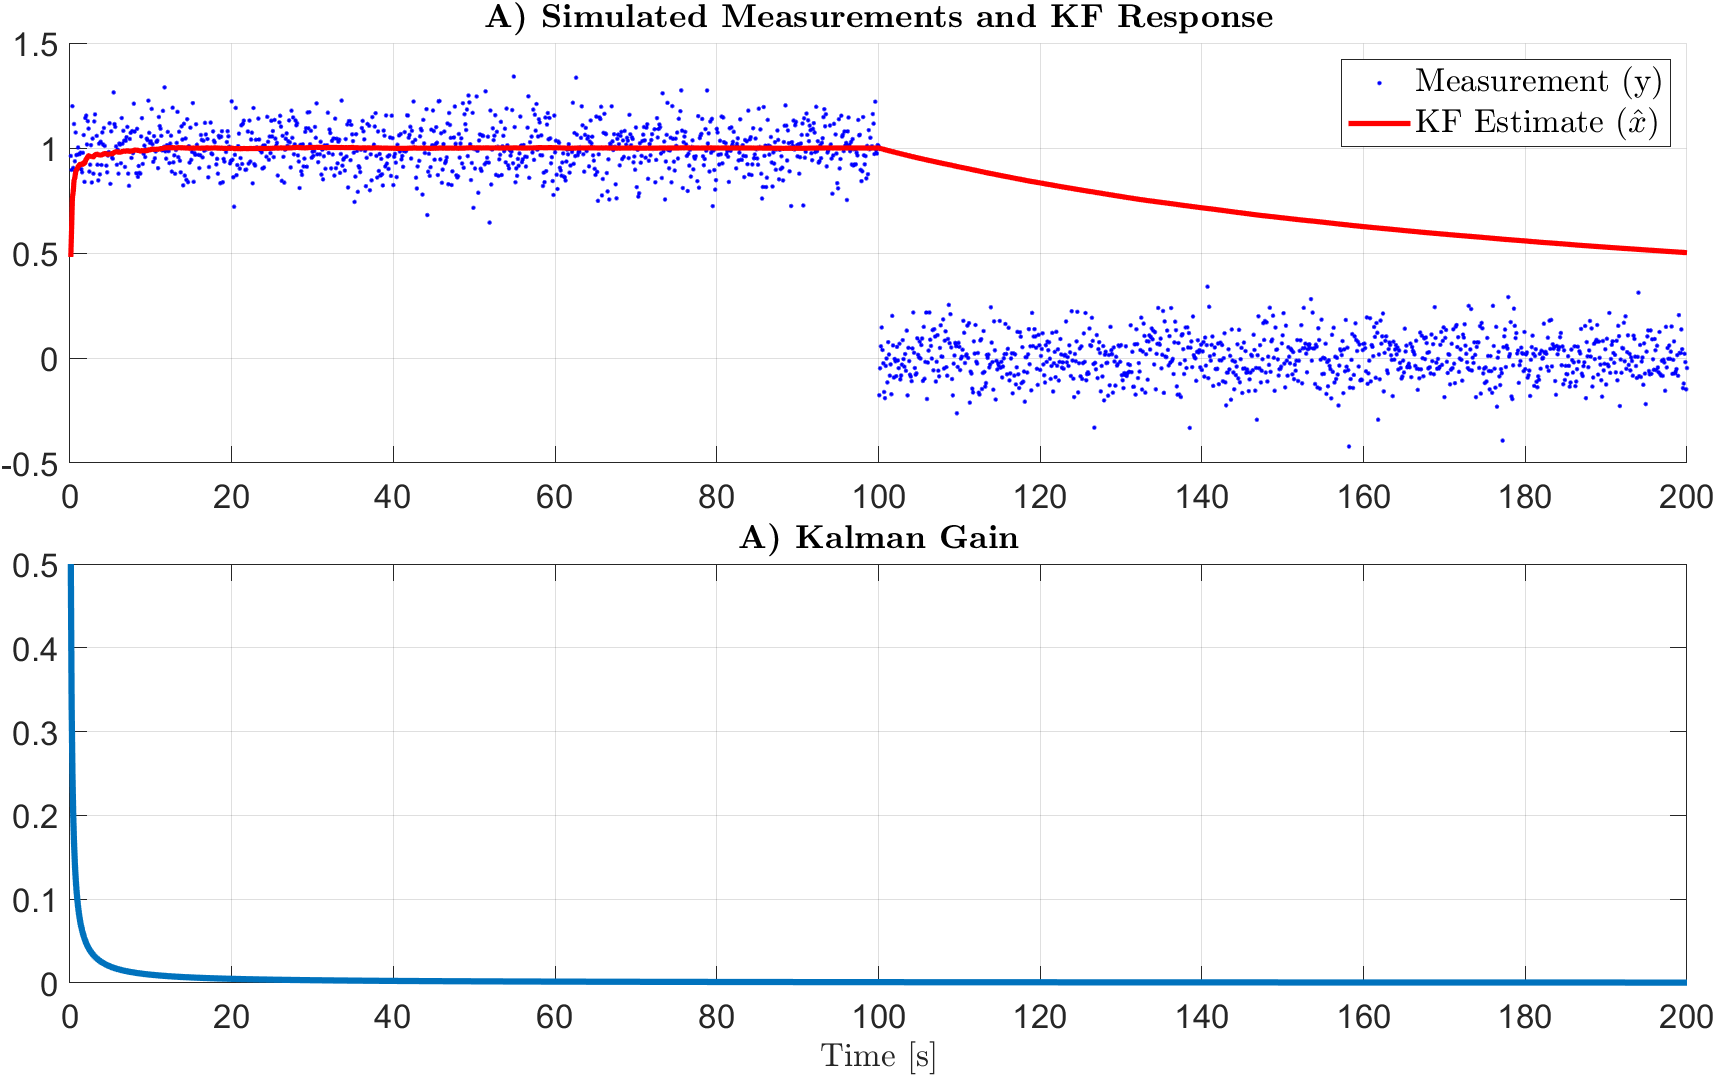
\includegraphics[width=0.8\textwidth]{p2_a.png}
    \caption{Kalman Filter 'Going to Sleep.'}
    \label{f:2.1}
  \end{figure}
  This figure also shows the Kalman Gain reaching a steady state values of 
  $L_{ss}=0.0005$ quickly. This can also be calculated and confirmed with 
  \emph{Equation \ref{eq:2.1}}.
  \begin{equation}
    \begin{split}
      P^{m}_{ss} &= \left[\left(A_d P^{m}_{ss} A_d^T + Q_d\right)^{-1} 
                + C R^{-1} C^T\right]^{-1} \\
      L_{ss} &= P^{m}_{ss}C^T R^{-1} \\
             &= 0.0005
    \end{split}
    \label{eq:2.1}
  \end{equation}

  % 2.B
  To tune the filter, four log spaced values of $Q = \begin{bmatrix} 0.1 & 0.01 
  & 0.001 & 0.0001 \end{bmatrix}$ were used as the process noise of the system. 
  The larger the process noise value, the quicker the filter was able to adapt 
  to the tracked the change in measured position, shown in \emph{Figure 
  \ref{f:2.2}}. It also shows that as $Q$ is increased $L_{ss}$ is also 
  increased as a byproduct. This indicates that more filtering (less smoothing) 
  is occurring as the dynamic model is trusted less.
  \begin{figure}[H]
    \centering
    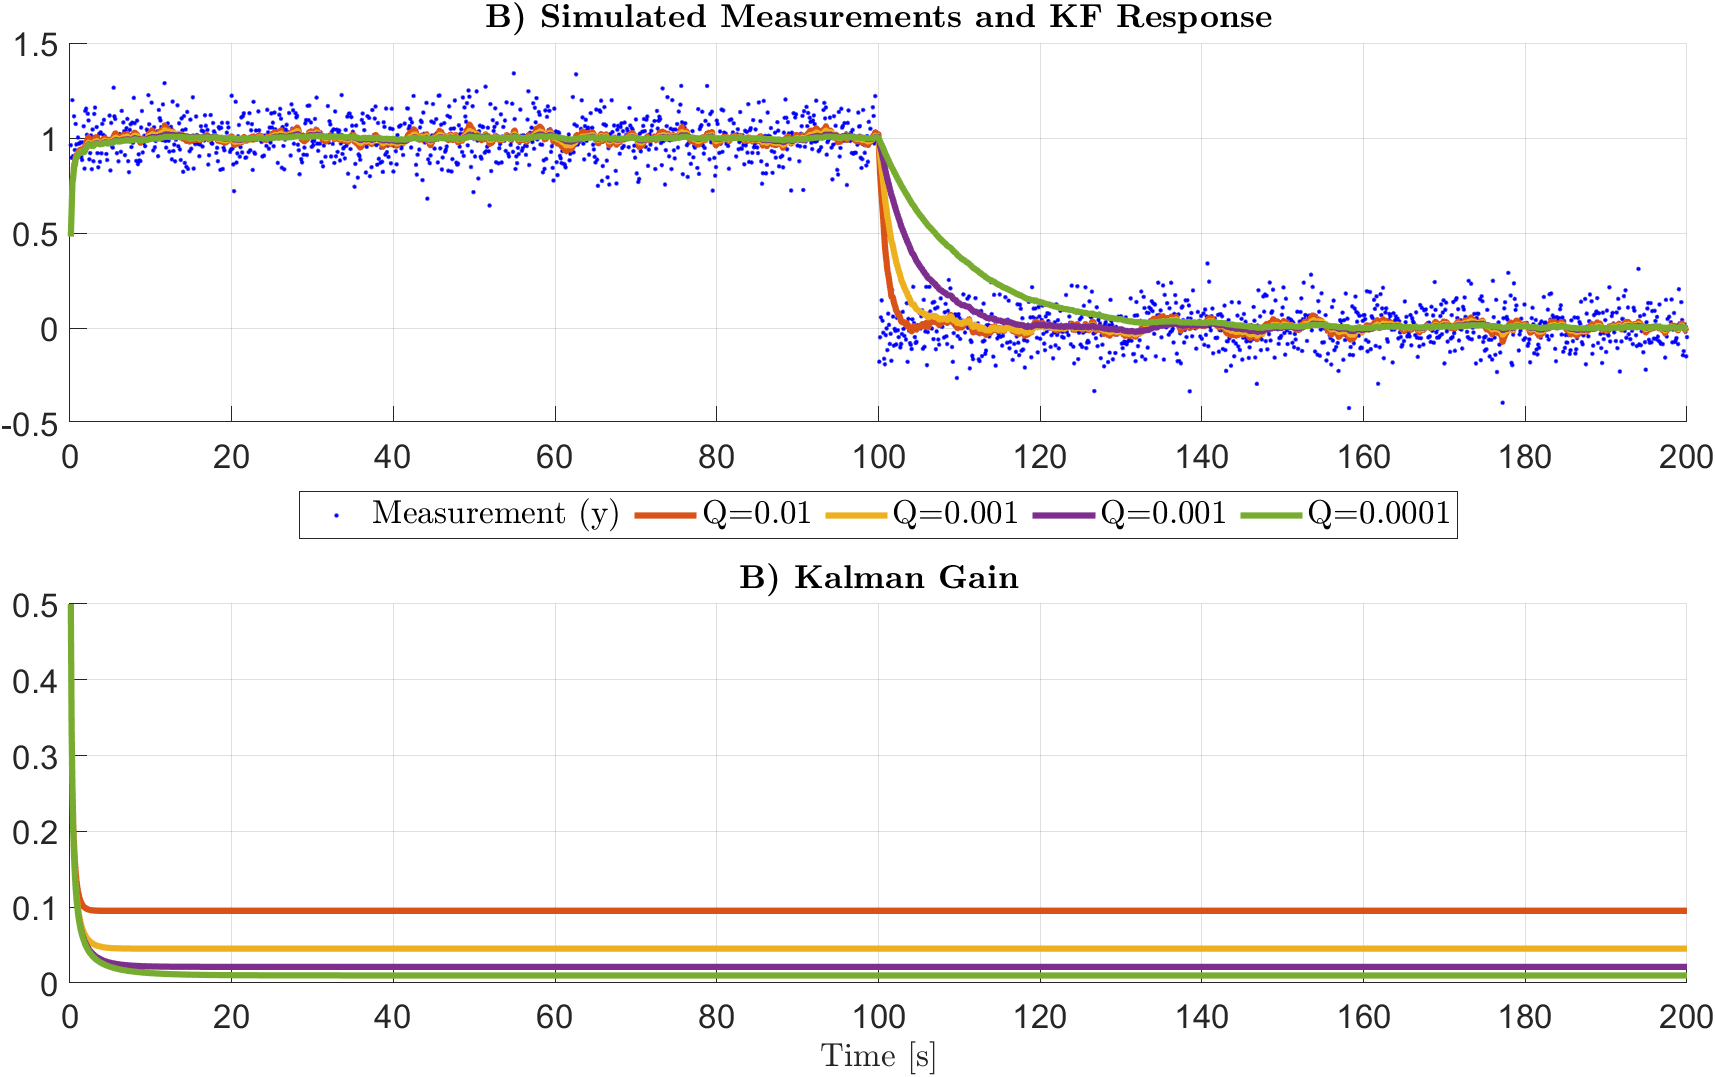
\includegraphics[width=0.8\textwidth]{p2_b.png}
    \caption{Filtered Position Estimate with a Varied Process Noise.}
    \label{f:2.2}
  \end{figure}

  % 2.C
  Choosing a process noise of $Q=0.1$, the MATLAB command $>>filter$ is used to 
  create a first order low pass filter as a comparison to the Kalman Filter we 
  created. Analyzing \emph{Figure \ref{f:2.3}}, it is obvious that the Low Pass 
  Filter is identical to the Kalman Filter. This is because once the Kalman 
  Filter reaches steady-state, it assumes the system is stationary and morphs 
  into a first order Low Pass Filter with the same pole placement.
  \begin{figure}[H]
    \centering
    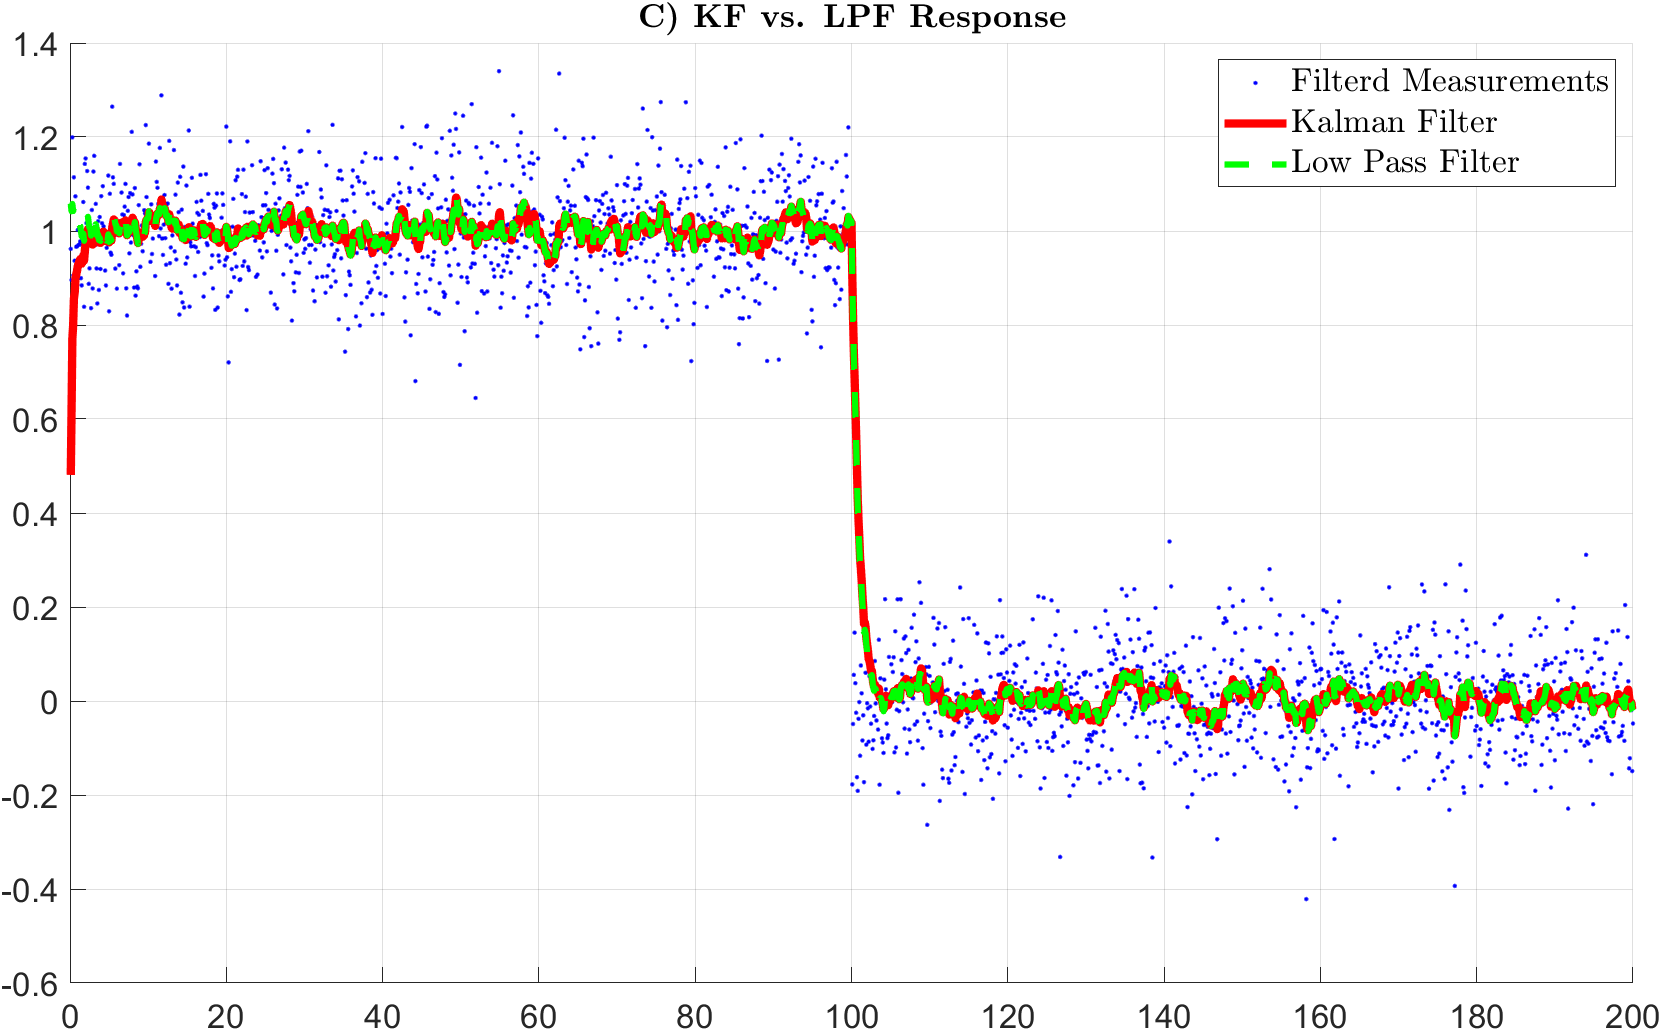
\includegraphics[width=0.8\textwidth]{p2_c.png}
    \caption{Kalman Filter v. First Order Low Pass Filter.}
    \label{f:2.3}
  \end{figure}

  \vspace{24pt}

  % PROBLEM 3
  \item Design a "Navigation" type Kalman filter to estimate the states [East, 
  North, Radar\_Bias, Psi, Gyro\_Bias]. Note: this is a non-linear problem that 
  requires an Extended Kalman Filter (EKF) to do correctly. However, we can solve 
  the problem in one of two ways: 
  \begin{enumerate}[(i)]
    \itemsep -2pt
    \item linearize the equations about the nominal operating point and produce 
    a constant A matrix for that operating point
    \item simply update the A matrix at every time step with our measurements or 
    estimates
  \end{enumerate}
  Download the data \emph{hw3\_3} from the website and run the filter sampled at 
  5 Hz.
  \begin{enumerate}[(a)]
    \itemsep -2pt
    \item How did you choose the covariance values for $Q_d$ (especially for the 
    radar and gyro biases).

    \item How does the bias estimation compare to a Least Squares Solution. How 
    does the bias estimate compare to the Recursive Least Squares solution if 
    you make the covariance ($Q_d$) of the bias estimates equal to zero.

    \item Integrate the last 40 seconds of data to see how well you have 
    estimated the biases. This can simply be done by “turning off” the 
    measurements in the observation matrix! Why do the bias estimates remain 
    constant during the 40 second "outage?"
  \end{enumerate}
  \vspace{10pt}

  \solution
  % 3.A
  For the time update, option \emph{ii} was chosen. This resulted in a nonlinear 
  state transition matrix that was updated every single iteration, and a linear 
  measurement mapping matrix as described in \emph{Equaion \ref{eq:3.1}} and 
  \emph{Equation \ref{eq:3.2}}.
  \begin{equation*}
    x_{k} = A_{k-1} x_{k-1}
  \end{equation*}
  \begin{equation}
    \begin{bmatrix} 
      \hat{E} \\ \hat{N} \\ \hat{\psi} \\ \hat{\dot{\psi}} \\ \hat{v} \\ \hat{b}_{\dot{\psi}} \\  \hat{b}_{v} 
    \end{bmatrix}_{k}
    = 
    \begin{bmatrix}
      1 & 0 & 0 & 0 & \Delta t \sin{(\hat{\psi}_{k-1})} & 0 & -\Delta t \sin{(\hat{\psi}_{k-1})} \\
      0 & 1 & 0 & 0 & \Delta t \cos{(\hat{\psi}_{k-1})} & 0 & -\Delta t \cos{(\hat{\psi}_{k-1})} \\
      0 & 0 & 1 & \Delta t & 0 & -\Delta t & 0 \\
      0 & 0 & 0 & 1 & 0 & -1 & 0 \\
      0 & 0 & 0 & 0 & 1 & 0 & -1 \\
      0 & 0 & 0 & 0 & 0 & 1 & 0 \\
      0 & 0 & 0 & 0 & 0 & 0 & 1 \\
    \end{bmatrix}
    \begin{bmatrix}
      \hat{E} \\ \hat{N} \\ \hat{\psi} \\ \hat{\dot{\psi}} \\ \hat{v} \\ \hat{b}_{\dot{\psi}} \\  \hat{b}_{v}
    \end{bmatrix}_{k-1}
    \label{eq:3.1}
  \end{equation}
  \begin{equation*}
    y_{k} = C x_{k}
  \end{equation*}
  \begin{equation}
    \begin{bmatrix} 
      E \\ N \\ \psi \\ \dot{\psi} \\ v 
    \end{bmatrix}_{k}
    = 
    \begin{bmatrix}
      1 & 0 & 0 & 0 & 0 & 0 & 0 \\
      0 & 1 & 0 & 0 & 0 & 0 & 0 \\
      0 & 0 & 1 & 0 & 0 & 0 & 0 \\
      0 & 0 & 0 & 1 & 0 & -1 & 0 \\
      0 & 0 & 0 & 0 & 1 & 0 & -1 \\
    \end{bmatrix}
    \begin{bmatrix} 
      \hat{E} \\ \hat{N} \\ \hat{\psi} \\ \hat{\dot{\psi}} \\ \hat{v} \\ \hat{b}_{\dot{\psi}} \\  \hat{b}_{v} 
    \end{bmatrix}_{k}
    \label{eq:3.2}
  \end{equation}
  With these matrices defined, the Kalman Filter can be applied as in 
  \emph{Equation \ref{eq:1.5}}. Both the measurement noise and process noise are 
  assumed to be uncorrelated between different states. The measurement noise was 
  defined as $1$ for measurement and the process noise on each estimate of the 
  measurement was $0.5$. These were chosen as smaller than the measurement noise 
  because the measurements seem to have little noise on them. For the biases, 
  since they should remain constant and are not measured,  no measurement noise 
  was applied and a small process noise of $0.001$ was used. $Q_d$ and $R$ are 
  defined in \emph{Equation \ref{eq:3.3}}. \\
  \begin{equation}
    \begin{split}
      R &= 
      \begin{bmatrix}
        1 & 0 & 0 & 0 & 0 \\
        0 & 1 & 0 & 0 & 0 \\
        0 & 0 & 1 & 0 & 0 \\
        0 & 0 & 0 & 1 & 0 \\
        0 & 0 & 0 & 0 & 1
      \end{bmatrix} \\
      Q_d &=
      \begin{bmatrix}
        0.5 & 0 & 0 & 0 & 0 & 0 & 0 \\
        0 & 0.5 & 0 & 0 & 0 & 0 & 0 \\
        0 & 0 & 0.5 & 0 & 0 & 0 & 0 \\
        0 & 0 & 0 & 0.5 & 0 & 0 & 0 \\
        0 & 0 & 0 & 0 & 0.5 & 0 & 0 \\
        0 & 0 & 0 & 0 & 0 & 0.001 & 0 \\
        0 & 0 & 0 & 0 & 0 & 0 & 0.001 \\
      \end{bmatrix} \\
    \end{split}
    \label{eq:3.3}
  \end{equation}
  \emph{Figure \ref{f:3.1}} shows the output of the Kalman Filter states 
  specified in the problem statement compared to their respective measurements.
  \begin{figure}[H]
    \centering
    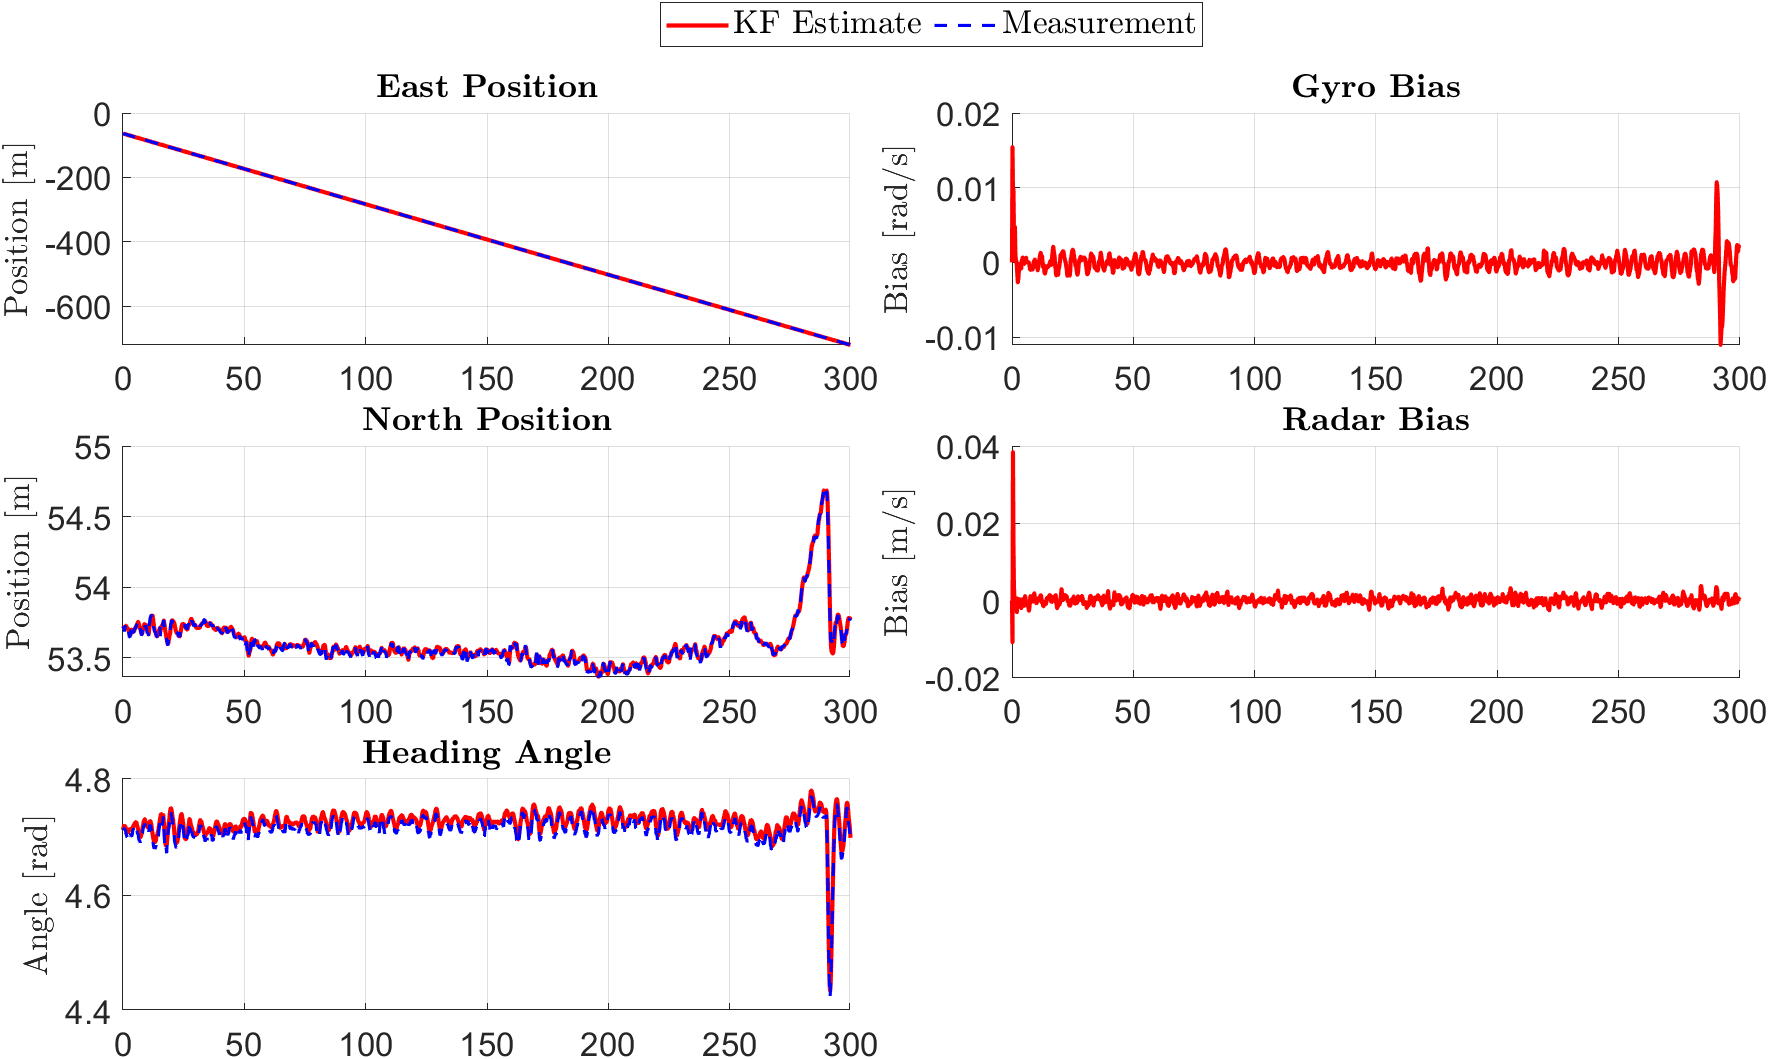
\includegraphics[width=0.9\textwidth]{p3_a2.png}
    \caption{Navigation Kalman Filter Estimates.}
    \label{f:3.1}
  \end{figure}

  % 3.B
  To run the system with least squares, the $C$ matrix defined in 
  \emph{Equation \ref{eq:3.1}} as the geometry matrix of the system. From here, the 
  psuedoinverse of the matrix is taken and multiplied by $y_k$ 
  (\emph{Equation \ref{eq:3.4}}).
  \begin{equation}
    x_{k} = (C^TC)^{-1}C^Ty_k
    \label{eq:3.4}
  \end{equation}
  For recursive least squares, a measurement propagation, similar to the Kalman 
  Filter measurement update, is used to recursively update the state 
  \emph{Equation \ref{eq:3.5}}.
  \begin{equation}
    \begin{split}
      Q_{k}^{-1} &= Q_{k-1}^{-1} + C^T R^{-1} C \\
      x_{k} &= Q C^T R^{-1} (y_k - C x_{k-1})
    \end{split}
    \label{eq:3.5}
  \end{equation}
  \emph{Figure \ref{f:3.2}} shows the least squares and recurve least squares 
  estimations of the system. The recursive least squares solution is considerably 
  worse than both the Kalman Filter and the regular least squares. This is because 
  recursive least squares assumes no dynamics, whereas the Kalman Filter expects 
  dynamics and least squares just estimates the most likely solution to the 
  information given. Due to this, the Kalman Filter outperforms both least 
  squares options in the estimation of the biases.
  \begin{figure}[H]
    \centering
    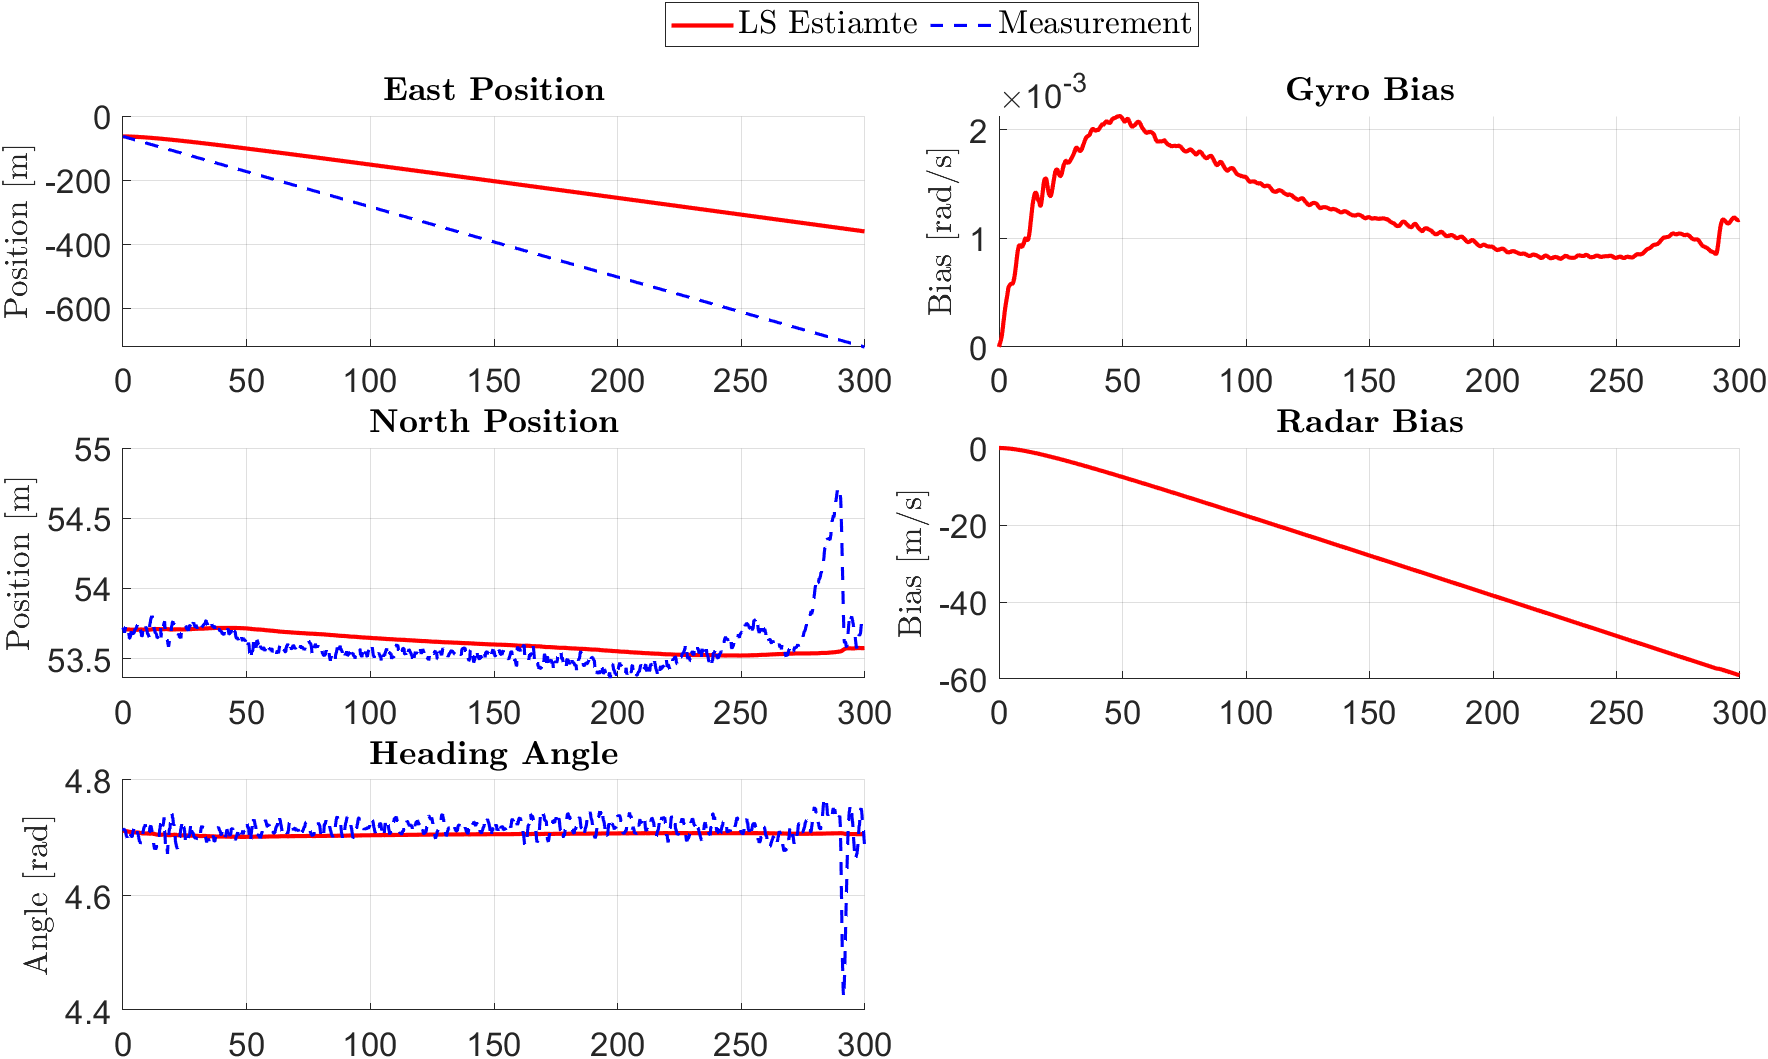
\includegraphics[width=0.9\textwidth]{p3_b2.png}
    \caption{Navigation Least Squares Estimates.}
    \label{f:3.2}
  \end{figure}

  % 3.C
  When solely integrating the system during for last 40 seconds, or the 
  'outage,' there is no measurement update or correction step. The measurement 
  update is crucial because it updates the covariance matrix that utilizes the 
  radar and gyroscope biases while filtering. Therefore, the bias estimates 
  remain constant throughout the 'outage.' \emph{Figure \ref{f:3.3}} shows the 
  last 50 seconds of the Kalman Filter designed in Part A where the measurement 
  update is turned off for the last 40 seconds.
  \begin{figure}[H]
    \centering
    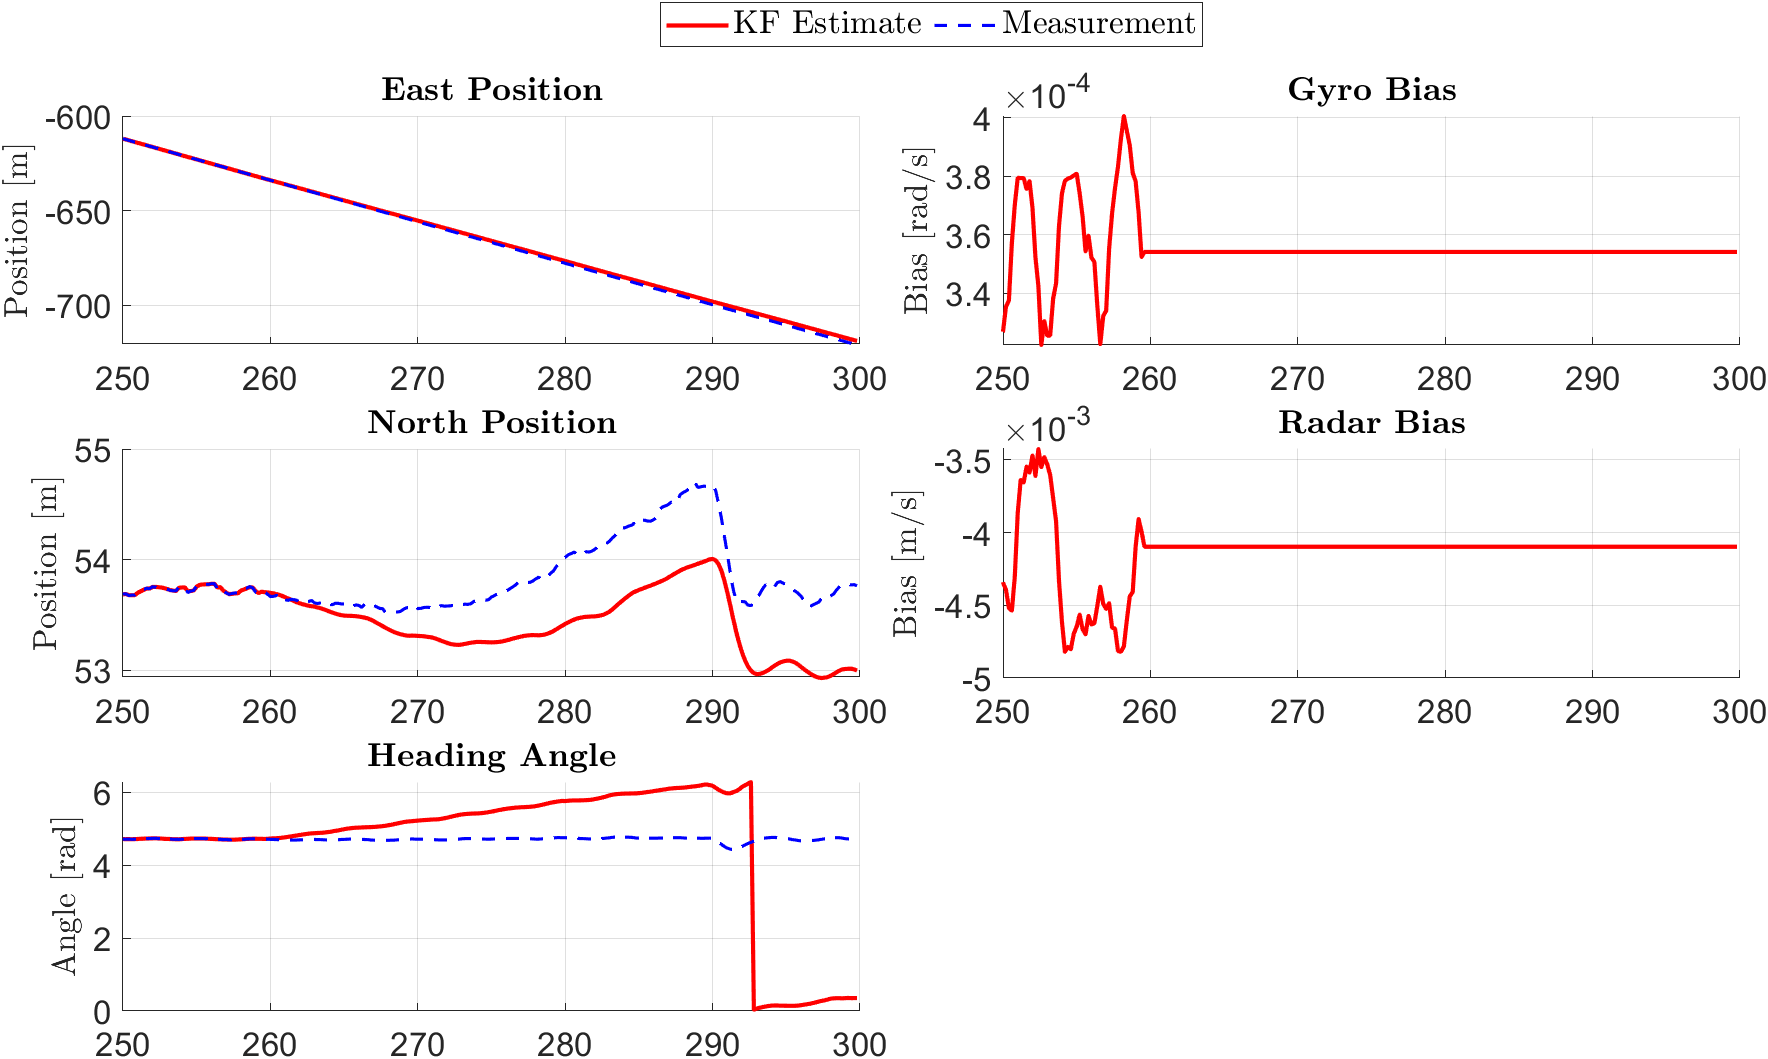
\includegraphics[width=0.9\textwidth]{p3_c2.png}
    \caption{Navigation 'Outage' Estimates.}
    \label{f:3.3}
  \end{figure}
  As shown, the bias estimates were tuned enough to provide good position 
  estimates but provided poor heading measurements.

  \vspace{24pt}

  % PROBLEM 4
  \item Estimator for Vehicle Dynamics. The yaw dynamics of a car (for a 
  stability control system) can be described by the following model (at 
  $25 m/s$):
  \begin{equation*}
    \begin{split}
      \dot{x} &= 
      \begin{bmatrix}
        -2.62 & 12 \\ -0.96 & -2
      \end{bmatrix}
      \begin{bmatrix}
        \dot{\psi} \\ \beta 
      \end{bmatrix}
      + 
      \begin{bmatrix}
        14 \\ 1
      \end{bmatrix} 
      \delta \\
      y_k &= 
      \begin{bmatrix}
        1 & 0
      \end{bmatrix}
      x_k + \nu_k
    \end{split}
  \end{equation*}
  Where:
  \begin{equation*}
    \begin{split}
      \dot{\psi} &= \text{Vehicle Yaw Rate} \\
      \beta &= \text{Vehicle Sideslip Angle} \\
      \delta &= \text{Steer Angle} \\
      \nu_k &= \text{Sample Sensor Noise}
    \end{split}
  \end{equation*}
  \begin{enumerate}
    \itemsep -2pt 
    \item Assuming we can only measure the yaw rate ($\nu_k \sim N 
    [0,(0.1)^2]$), design a Kalman filter to do full state estimation (select a 
    reasonable $Q_d$). Provide a unit step steer input and estimate both states. 
    On one page plot the actual states and estimated states (use 
    $subplot(2,2,n)$ for each of the two states). Where are the steady state
    poles of the estimator?

    \item Now, somebody has loaded the trunk of the vehicle with bricks, 
    changing the CG of the vehicle so now the actual model (at 25 m/s) is:
    \begin{equation*}
      \begin{split}
        \dot{x} &= 
        \begin{bmatrix}
          -2.42 & 4 \\ -0.99 & -2
        \end{bmatrix}
        \begin{bmatrix}
          \dot{\psi} \\ \beta
        \end{bmatrix} 
        +
        \begin{bmatrix}
          18 \\ 1
        \end{bmatrix}
        \delta \\
        y_k &= 
        \begin{bmatrix}
          1 & 0
        \end{bmatrix}
        x_k + \nu_k
      \end{split}
    \end{equation*}
    NOTE: We do not know that somebody has loaded the trunk and that the C.G.
    has changed, therefore we must use the model for \emph{part a} in our Kalman 
    Filter. Redo \emph{part a}. Can you estimate the slip angle correctly? Try 
    various $Q_d$.

    \item Now lets say we have a noisy measurement of the slip angle ($\eta_k 
    \sim N[0,(0.5)^2]$):
    \begin{equation*}
      y_k = 
      \begin{bmatrix}
        1 & 0 \\ 0 & 1
      \end{bmatrix}
      x_k + 
      \begin{bmatrix}
        \nu_k \\ \eta_k
      \end{bmatrix}
    \end{equation*}
    Assuming the sensor noises are uncorrelated, what is $R$?

    \item Redo \emph{part a}. What is the effect of changing the element of 
    $Q_d$ associated with the slip angle estimate. What must $Q_d$ equal to 
    ensure an unbiased estimate of the states. How much filtering does that 
    provide?
  \end{enumerate}
  \vspace{10pt}

  \solution
  % 4.A
  To run the Kalman Filter, the system must first be discretized 
  (\emph{Equation \ref{eq:4.1}}).
  \begin{equation}
    \begin{split}
      A_d &\approx eye(2) + A \Delta t = 
      \begin{bmatrix}
        0.738 & 1.20 \\ -0.096 & 0.80
      \end{bmatrix} \\
      B_d &\approx B \Delta t = 
      \begin{bmatrix}
        1.4 \\ 0.1
      \end{bmatrix} \\
      C_d &= C = 
      \begin{bmatrix}
        1 & 0
      \end{bmatrix}
    \end{split}
    \label{eq:4.1}
  \end{equation}
  The measurement noise is provided as $R=0.1^2=0.01$ and the process noise was 
  tuned to be:
  \begin{equation*}
    Q_d = \begin{bmatrix} 2 & -1 \\ -1 & 0.5 \end{bmatrix}
  \end{equation*}
  Using these parameters along with the one given in the problem statement, we 
  can estimate the yaw rate and sideslip angle of the car 
  (\emph{Figure \ref{f:4.1}}). From the Kalman Filter, with a constant 
  $Q_d$ and $R$, we get the discrete poles of the steady-state Kalman Filter to 
  be:
  \begin{equation*}
    poles = 
    \begin{bmatrix}
      -0.013 + 0i & 0.533 + 0i
    \end{bmatrix}
  \end{equation*}
  \begin{figure}[H]
    \centering
    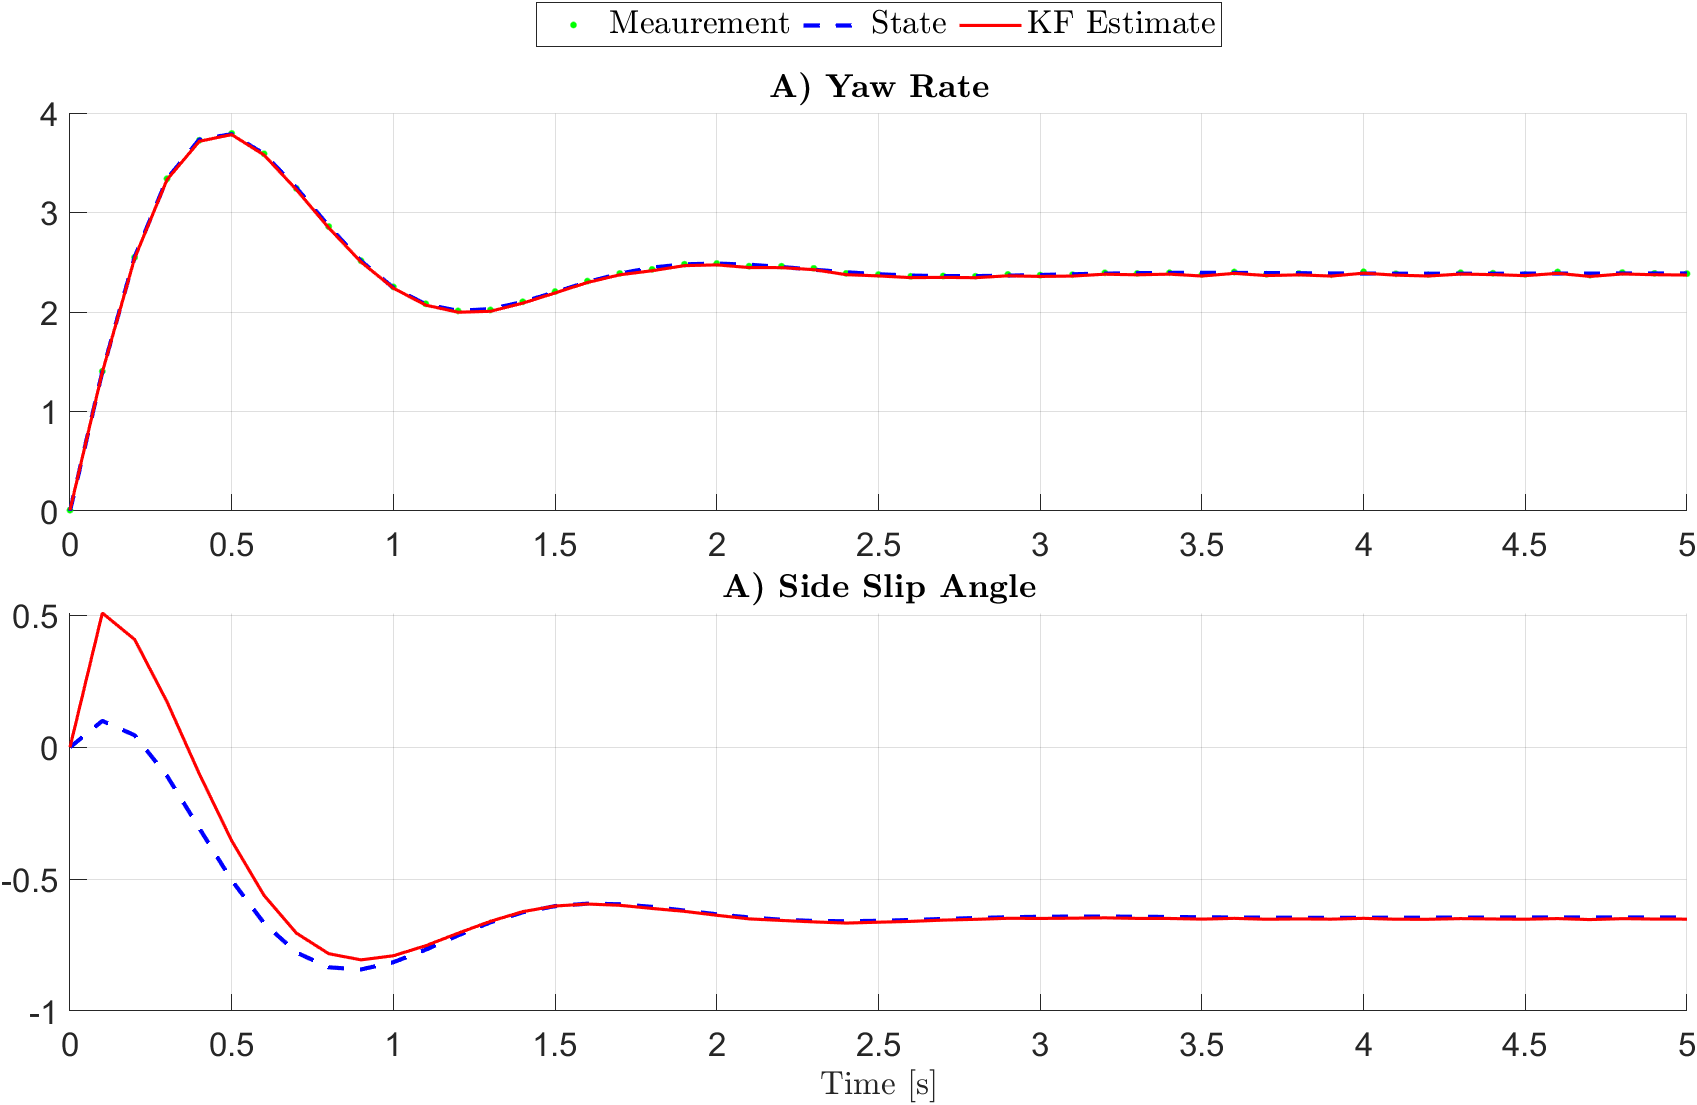
\includegraphics[width=0.8\textwidth]{p4_a.png}
    \caption{Vehicle Dynamics Kalman Filter Estimation.}
    \label{f:4.1}
  \end{figure}
  It is shown that the estimate of the sideslip angle is of similar accuracy to 
  the yaw rate estimation. This is because the sideslip angle of the car is not 
  directly observable based on the current measurement matrix.

  % 4.B
  When the dynamic model of the system is slightly altered, the process noise 
  matrix can also be slightly altered to match the new system. However, all 
  other matrices are kept the same as in Part A. The new process noise matrix 
  and discrete poles are:
  \begin{equation*}
    \begin{split}
      Q_d &= \begin{bmatrix} 3 & -1.2 \\ -1.2 & 0.5 \end{bmatrix} \\
      poles &= \begin{bmatrix} -0.099+0i & 0.639+0i \end{bmatrix}
    \end{split}
  \end{equation*}
  \begin{figure}[H]
    \centering
    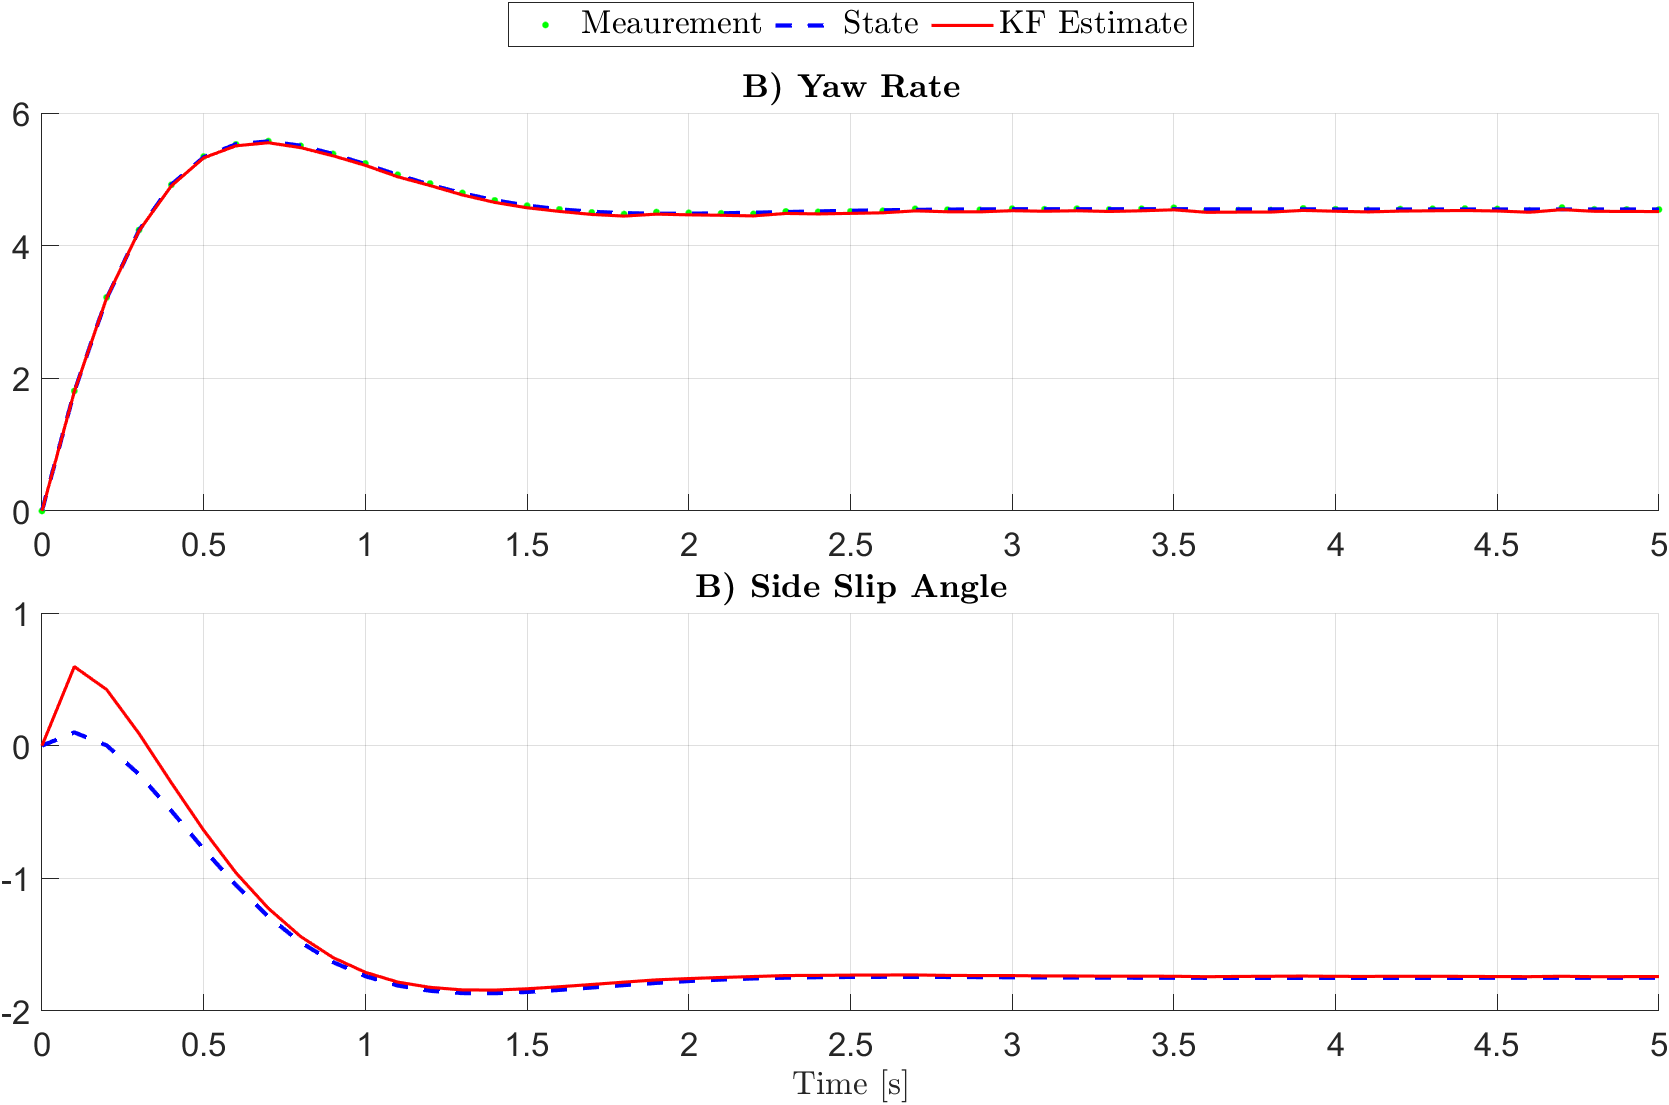
\includegraphics[width=0.8\textwidth]{p4_b.png}
    \caption{Vehicle Dynamics Kalman Filter Estimation with Altered Dynamic Model.}
    \label{f:4.2}
  \end{figure}
  As shown in \emph{Figure \ref{f:4.2}}, with the altered process noise, the 
  steady state errors are approximately the same as in Part A.

  % 4.C
  Adding a noisy measurement of slip angle with the statistics defined in the 
  problem statement changes the measurement noise and new geometry matrix to be:
  \begin{equation*}
    \begin{split}
      R &= \begin{bmatrix} 0.01 & 0 \\ 0 & 0.25 \end{bmatrix} \\
      C &= \begin{bmatrix} 1 & 0 \\ 0 & 1 \end{bmatrix} \\
    \end{split}
  \end{equation*}

  % 4.D
  As we can see from \emph{Figure \ref{f:4.3}}, the effect that adding a second 
  measurement has on the estimation is substantial. It is obvious that is makes 
  the estimation of the parameter much more noisy. However, the same process 
  noise matrix from Part A does not work such that the process noise values 
  must be significantly smaller to work for this system. The addition of the 
  direct measurement of sideslip allows much more leniency in the design of the 
  system. Decreasing the value of $Q_d$ allows for more smoothing by reducing 
  the apparent noise. The new values of $Q_d$ and the steady state Kalman Filter 
  poles are:
  \begin{equation*}
    \begin{split}
      Q &= \begin{bmatrix} 0.2 & -0.01 \\ -0.01 & 0.02 \end{bmatrix} \\
      poles &= \begin{bmatrix} 0.080+0i & 0.362+0i \end{bmatrix}
    \end{split}
  \end{equation*}
  \begin{figure}[H]
    \centering
    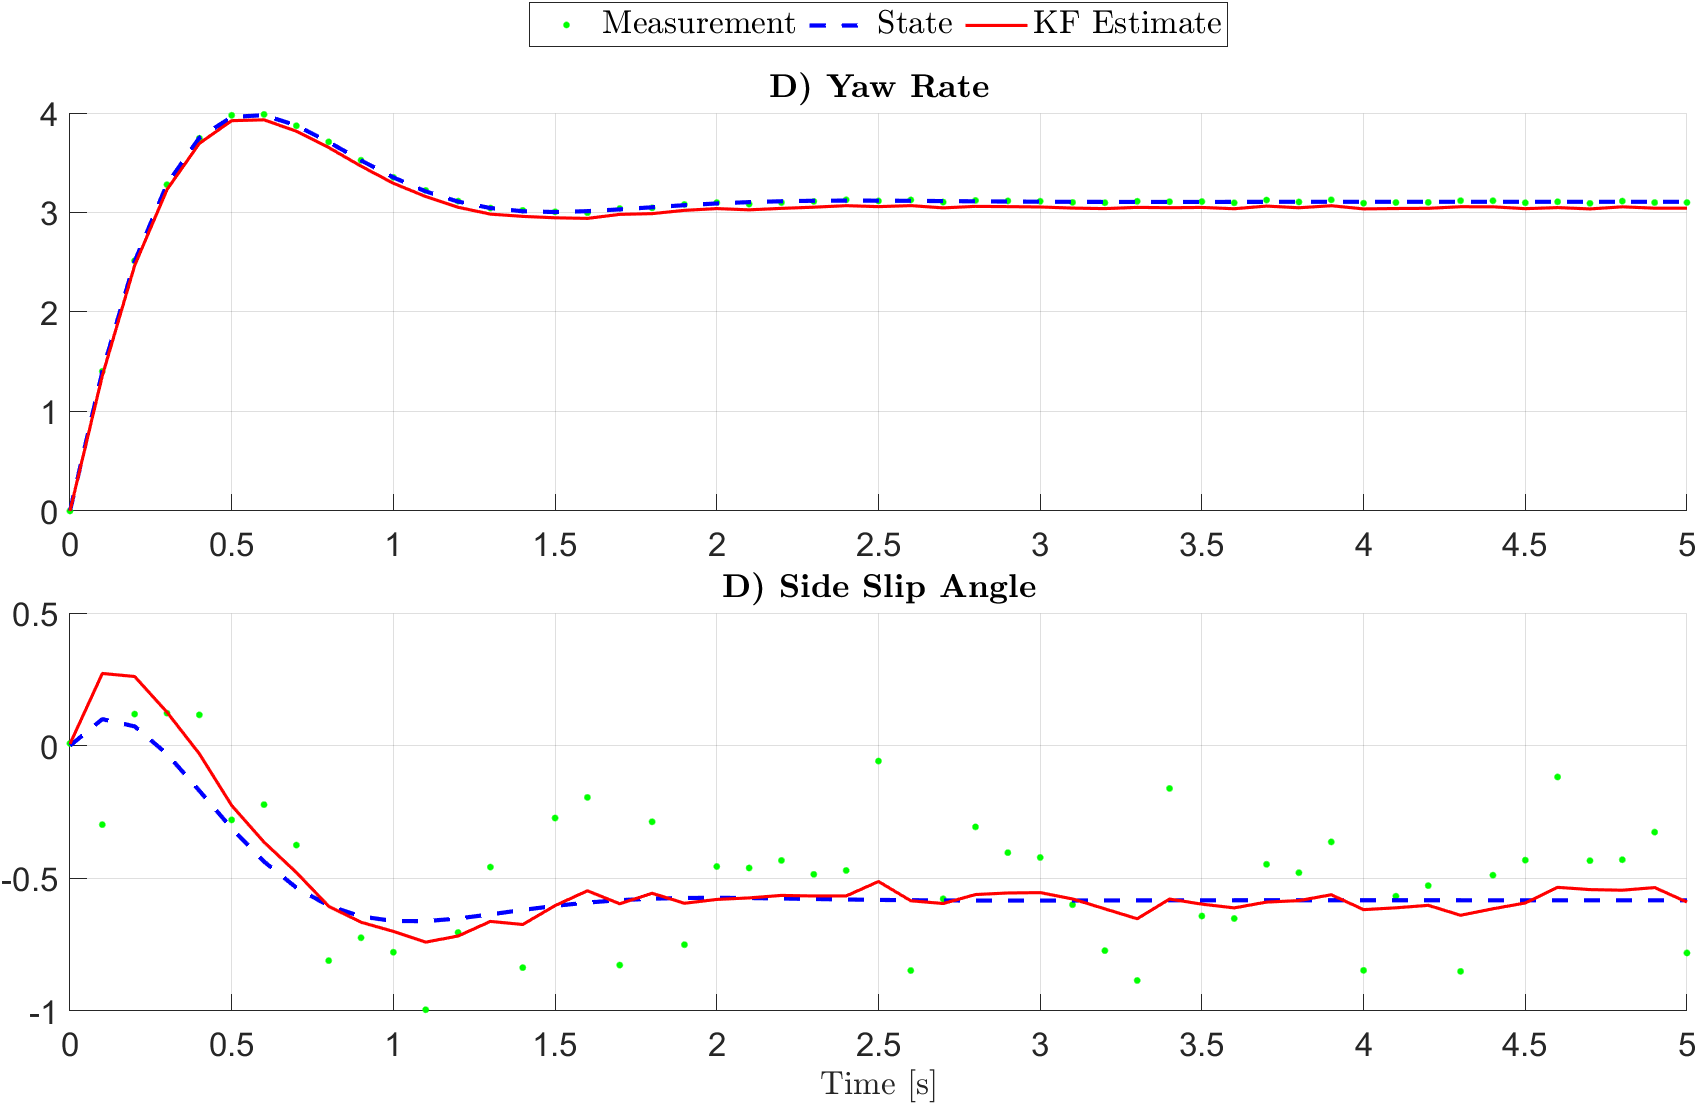
\includegraphics[width=0.85\textwidth]{p4_d.png}
    \caption{Vehicle Dynamics Kalman Filter with the Addition of Measurements of Sideslip.}
    \label{f:4.3}
  \end{figure}
  Overall, a more realistic estimate of sideslip is achieved but at the cost of 
  increased noise.

\end{enumerate}

\end{document}